\section{Abstract}
\todo{the whole thing :(}

\section{Intro}
\label{sec:intro}

%%State of the world
Disaggregated computing promises higher resource density, increased
power-efficiency, and flexible application scalability in datacenters.
While enticing, these benefits have remained mostly untapped due to
the proportionally large overhead of accessing remote resources.
Nowhere is this disparity more noticeable than remote memory.
Separating CPUs last level cache from their main memory incurs at
least a 20x overhead (approximately 50\textit{ns} to 1\textit{us}).
The cost is only acceptable for select asynchronous workloads, such as
paging out infrequently touched data~\cite{infiniswap,legoos,leap},
but are entirely unrealistic when multiple CPUs require consistency
for frequent reads and writes to shared remote memory.

A large body of work has investigated how to design high performance
RDMA key value stores, and RPC
frameworks~\cite{cell,sonuma,storm,farm,herd,erpc}. However, they
require that a CPU be coresident with remote memory to coordinate RDMA
access and keep their remote data structures consistent. In the case
of pure resource disaggregation no CPUs are coresident with remote
memory. This architectural difference requires new techniques and
algorithms to achieve similar functionality and performance. 

Some research has been done into the requirements for resource
disaggregation, specifically with regard to network, and memory
requirements~\cite{requirements, aguilera2019designing, disandapp,
amanda-hotnets}. Few have been tested practically and some require
non-existent hardware primitives. Those that have been constructed are
first attempts at exposing remote memory to clients without the
expectation of remote CPUs~\cite{reigons, clover}. Both Remote
Regions~\cite{reigons} and Clover~\cite{clover} are designed to use
remote memory with a read heavy workload on any shared resources.
%%
Their reason for avoiding writes is fundamental: concurrent consistent
writes to remote memory are expensive. Lock acquisition and revocation
requires multiple round trips which devastates throughput.  Even with
an intelligent concurrent algorithm to opportunistically avoid lock
acquisition the problem is pervasive due to the natural concurrency
and relatively high latency of remote memory.
%%
In the opportunistic case write conflicts due to inconsistencies in
local caches occur frequently when resources are contested.
Figure~\ref{fig:conflicts} shows the number of concurrent conflicting
writes to shared resources as the number of clients requesting the
resources are increased.

\begin{figure}
    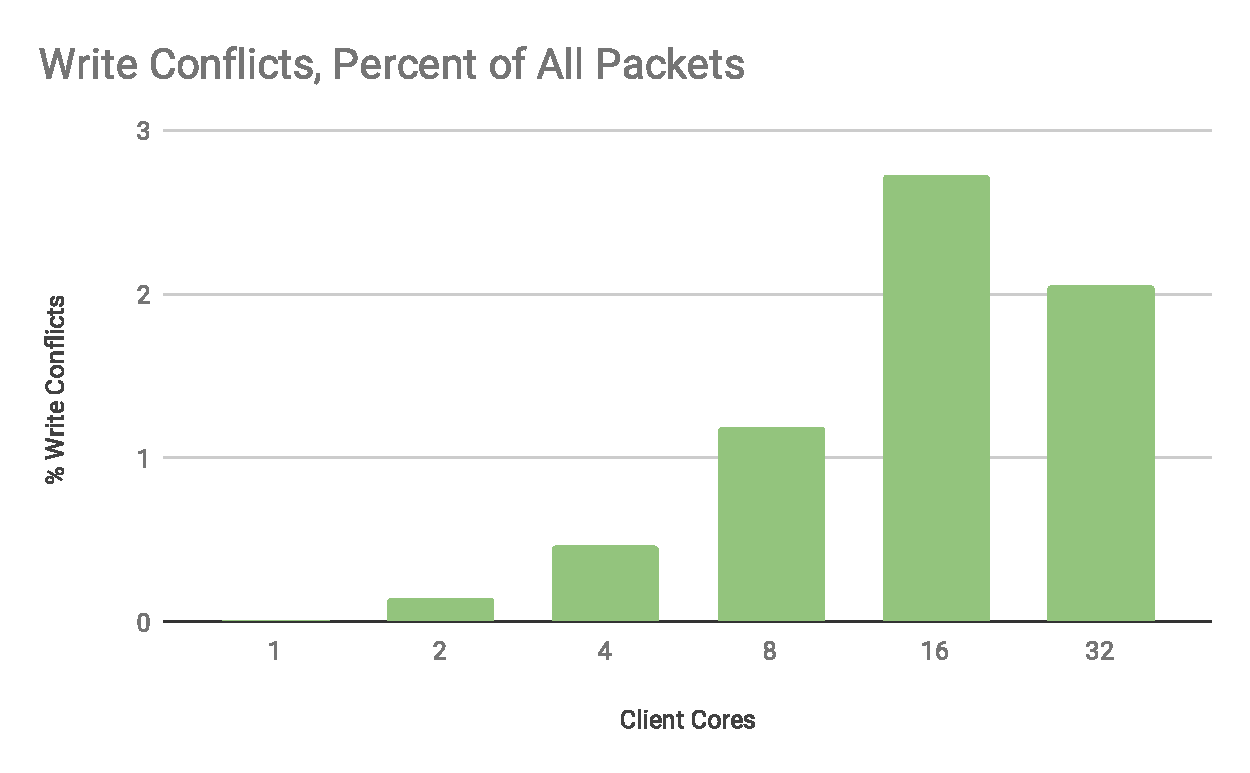
\includegraphics[width=0.45\textwidth]{fig/write_conflicts.pdf}
    \caption{Clover write conflicts grow with the number of clients
    (50\% write zipf 0.99 distribution)\todo{redo with 64 cores and
    writes only}}
    \label{fig:conflicts}
\end{figure}


In clovers specific case its throughput is severely degraded under
write heavy workloads. Figure~\ref{fig:clover_tput} shows clovers
reported throughput drop when subjected to a 50\% write workload.

\begin{figure}
    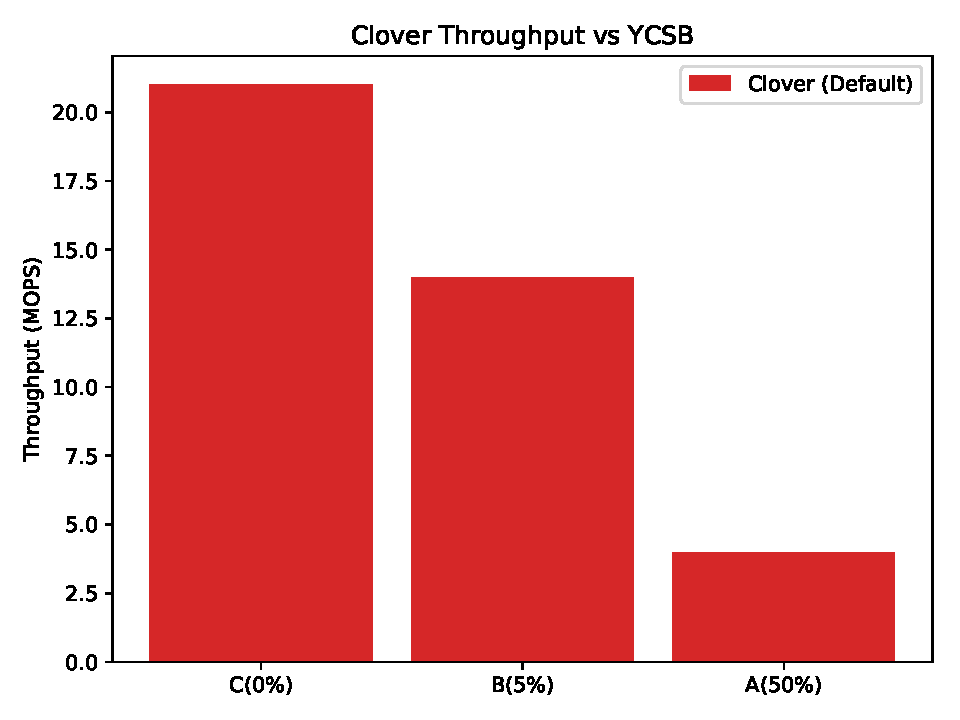
\includegraphics[width=0.45\textwidth]{fig/clover_tput.pdf}
    \caption{Clover throughput degradation as a function of write
    workload\todo{redo on my setup for consistent ops/s}}
    \label{fig:clover_tput}
\end{figure}


This work makes the contention that a programmable TOR is an ideal
centralized point at which to resolve remote memory conflicts. Prior
work has suggested the need for a distributed memory
controller~\cite{disandapp}, but none have been built or proposed with
existing hardware. We observe that in a disaggregated setting if all
remote reads and writes are performed within a rack using RDMA a TOR
in a unique position to observe every memory operation.  This fact
allows it to act as a centralized serialization point, where the last
instance of read/write concurrency are the memory attached egress
ports of the switch.  Figure~\ref{fig:overview} illustrates the
organization of a disaggregated rack, and highlights different
proposed points of coordination for reads and writes.

As a proof of concept we interpose on the Clover protocol and resolve
write conflicts in its datapath. Our conflict detection algorithm uses
knowledge of Clovers remote data structures to detect write conflicts
using a small amount of cached state (only a few bytes per key value
pair). Conflict resolution is performed directly on the in flight RDMA
packets by steering their destination virtual addresses to the most up
to date read and write locations in Clovers key value store. This
technique is complete, in that it resolves all read and write
conflicts given that it caches all keys. As in network SRAM is expense
we show that our technique can trade completeness for memory savings
while still achieving performance gains. Our preliminary evaluation
shows maximal throughput gains of 1.42x (tracking all reads and
writes), and gains of 1.34x when correcting conflicts on the top 8
keys of a zipf request distribution using only 128 bytes of in network
memory.

\begin{figure*}
      \centering
      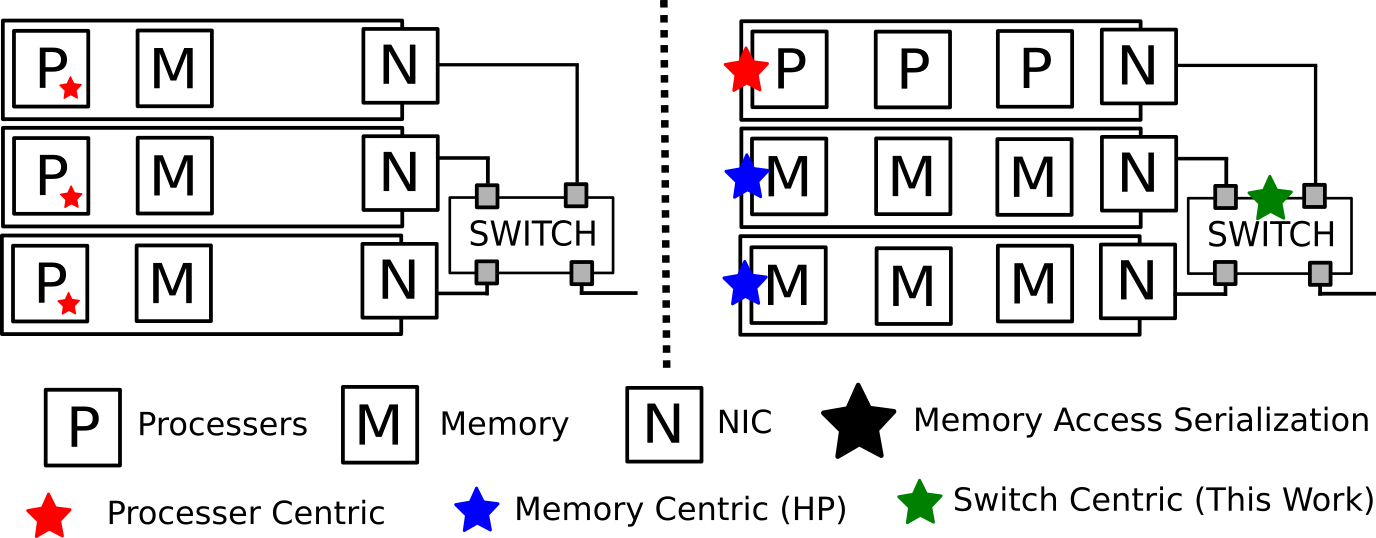
\includegraphics[width=0.95\textwidth]{fig/overview.png}
      %%
      \caption{~\todo{redo diagram to remove memory centric
      organization (it's a pipe dream)}
      Anatomy of a disaggregated rack. On the left a
      traditional rack with processors colocated with their memory
      interconnected by a switch. On the right is a high density
      disaggregated rack with processors separated from their memory
      by a top of rack switch. Stars mark locations for memory access
      serialization. Red denotes traditional processor centric
      serialization~\cite{memc3, cell, sonuma, storm, clover}, blue marks a
      memory centric architecture~\cite{aguilera2019designing}, and
      green marks a switch centric solution similar in spirit to
      proposed middle box solutions~\cite{254120}.
      \label{fig:overview}
      %%
      }
\end{figure*}



\section{Clover}

%%
Clover proposes that disaggregated data structures separate their
computational concerns into distinct responsibilities. Mainly memory
servers, which passively accept RDMA requests, Clients which issues read and
writes to the remote memory banks, and Metadata severs which
centralize and keep consistent the shared metadata of the disaggregated
data structures.

Through their experimentation they find that ideal throughput is
gained by placing client shared metadata out of datapath entirely, and
updating it opportunistically. Placing a metadata coordinator in the
datapath quickly leads to a performance bottleneck. Their algorithm
optimizes read operations, and allows for lockless line rate reads. In
the presence of writes however clovers operation throughput decreases
due to contention. When concurrent writes contest the same data a race
occurs in which the fastest writer wins. Write operations require two
messages, a data update (RDMA WRITE) and a check and set (RDMA CNS)
which updates old data to point to the new version. During this two
RTT operation any concurrent write to the same key will cause a
conflict. The slower writers will fail, and must retry their writes
after searching through clovers remote data structure for the next
write location to update their local cache (an operation known as
pointer chasing). On write heavy workloads these race conditions
happen frequently as illustrated in Figure~\ref{fig:conflicts}, which
leads to a sharp decrease in throughput.



%% what are we discussing
Clover's write strategy is opportunistic, it attempts to make updates
without acquiring locks, in the hope that no conflicts occur. When
they do occur it's just job of the writer to reconcile the conflict.
This opportunism amortizes the cost of lock acquisition when
contention is low, providing average case O(1) read/write and is used
in many high throughput concurrent data structures.

%%
We propose a middle ground between prior centralized approaches, and
clover's out of datapath metadata separation. Our insight is that by
caching small amount of a disaggregated data structures metadata in a
centralized location, write conflicts can be resolved at line rate in
the data path allowing for conflict free full read and write
throughput of disaggregated data structures. Using Clover as a
platform to prove our concept we design a lightweight middle box
algorithm which intercepts clovers RDMA read and write request, caches
a small amount (64 byte per key) amount of structural meta data and
resolves write conflicts by adjusting the destination RDMA address of
the writes. Our algorithm is implemented in DPDK, but is designed to
have low memory and computational overhead making it ideals for
network devices such as programmable switches and NICs.


%% The high level pitch about remote memory.
%Far memory projects typically have a remote CPU which is used to
%coordinate access to remote resources (cite all object systems). In a
%disaggregated system there is no remote CPU, therefore the coordination
%of reads and writes to remote locations must be done locally. For
%performance local caches of remote resources can be used to organize
%access to remote resources. For data structures which require
%consistency this creates a problem as stale caches can lead to data
%structure corruption.

\section{Our System}

Our system caches metadata for remote data structure on centralized
networking devices. Our prototype is implemented in DPDK, however our
algorithm could be implemented on a programmable switch or
programmable NIC as long as it sees all requests to remote memory. 
%% kinds of devices
A programmable TOR or our DPDK switch (which behaves as one) is ideal
for rack scale disaggregated structures that potentially span multiple
memory servers, while a programmable NIC implementation would be
limited limited to the memory server it is attached to. 

%%Technique example
The purpose of our technique is to resolve write conflicts to remote
memory. As an example of a conflict take a linked list implemented as
a remote data structure with a single operation, \textit{appendTail}.
This operation ensures that the next write to the data structure
writes to the tail of the linked list. This operation requires two
steps.  First a writer sends and RDMA write to the remote memory which
writes the data value for the new tail. After the data is written a
second operations consisting of an RDMA check and set (CNS) is issued
to the old tail which replaces it's NULL next pointer with the address
of the newly written tail.

This operation succeeds every time in the single threaded case as the
tail of the linked list is never moved by another process. Consider
instead the multi-threaded case in which two writer both attempt to
execute \textit{appendTail} concurrently. Both issue their first write
to remote memory successfully and then attempt to run an RDMA CNS on
the tail of the old list. This results in a race condition where one
process succeeds, and the other will fail. The process which executes
the CNS second fails because rather than finding a tail with a next
value of NULL, it finds the now penultimate member of the linked list
which now points to the value issued by the process which won the
race. 

The process which lost the race now needs to engage in \textit{Pointer
chasing}. It must iterative issue reads of the linked list until it
finds the location of the new tail. At which point it can reissue a
CNS to make the new tail point to it's value. This reconciliation
algorithm of pointer chasing must be run each time a conflict occurs.
For highly contested structures, the number of retries can grow
quickly, leading to large and unpredictable tail latencies.

In the case of clover this exact scenario occurs when key are write
contested. Their experiments with a zipf distribution on their keys
sees a \todo{5x} reduction in throughput.

%% What do we actually do
If a central arbiter where to observer the writes to this linked list
it would notice that the second CNS does not need to fail, it simply
needs to be redirected to point at the new tail of the list. 
%%
Our contention is that such a coordinator can be implemented in
network with minimal overheads to significantly improve the write
throughput. Using data structure specific information the coordinator
can cache recent writes, and steer concurrent ones to locations which
will result in successful operations and maintain the correctness of
the remote data structure.

In the case of clover we cache the tail of the linked list for each
key in clovers key value store. This results in an \textit{O(n)}
overhead where n is the number of keys. In our case for a key value
store consisting of 10k keys we need to store a key mapping and value
for each (both 64 bits) resulting in a total in network storage of
80KB. Note that this O(n) overhead is only a small fraction of clovers
metadata. Each key has a versioned history of writes, however only the
tail of the list is required to accelerate writes.

\textbf{Modifying RDMA in flight:}\sg{added long explicit explanation
about RDMA and conflict fixing} Interposing on an RDMA protocol is non
trivial. One solution (evaluated in as Clover
pDPM-central~\cite{clover}) would be to use an RDMA enabled middlebox
to setup connections between the clients and the memory servers which
would reissue RDMA request to the consistent locations. This solution
is impossible for a switch as it lacks the capabilities and resources
to establish RDMA connections. Further it has been demonstrated to be
a performance bottleneck. Our algorithm interposes on RDMA requests
transparently without storing any explicit RDMA state, or establishing
connections.

When RDMA write requests are issued our algorithm stores the locations
of the virtual addresses of the writes for each client thread. These
writes are marked as \textit{outstanding}. Outstanding writes are
writes which have been made to remote memory, but which have not yet
been made consistent in clover. Outstanding writes are not yet
connected to clovers key linked lists and therefore cannot be read by
other clients. Following an outstanding write clients will issue an
RDMA CNS which points the tail of the last committed write to the last
outstanding write the client issued, making it the new tail of the
list. Our algorithm detects the existence of a conflict when there is
more than one outstanding write for a given key. In addition to
tracking outstanding writes per client, our algorithm tracks the last
CNS issued to each key. This CNS marks the true tail of a keys linked
list. When a CNS for an outstanding write is seen, and the virtual
address of it's CNS points to an old tail, it's virtual address is
modified in flight (without the knowledge of the issuing client) to
point to the true tail of the list. The cached latest version of the
key is then updated to point to the address the CNS was directed to.
Clover clients learn the updated locations using their default read
algorithm.

RDMA packets are not intended to be modified in flight, and care must
be taken no to corrupt them. RDMA invariant CRCs are calculated at the
time of sending and are designed to ensure the integrity of the
payload. When CNS packets are modified their ICRC must be recalculated
or the modified packet will be rejected the RDMA hardware on the
receiving NIC. FPGA implementations of RDMA ICRC have been built in
the past~\cite{Mansour_2019}, the required CRC calculation is
identical to ethernet CRC, with the requirement of additional header
injection and field masking. We believe that this algorithm can be
implemented efficiently on a programmable switch.

\section{Evaluation}

Our experimental setup consists of 4 machines each with two sockets
equipped Intel Xeon E5-2640 CPU's and 265GB of main memory evenly
spread across two NUMA domains. Each machine has a Mellanox ConnectX-5
100Gbps NIC installed in a 16x PCIe slot. Each server is
interconnected via a 100Gbps Mellanox Onyx Switch. We designate a
single server to run as both the memory server (MS) and as the meta
data server (DN). Two machines are configured as clients, and a single
machine acts as a programmable switch.

All clover servers are configured using default routing settings.
Clients are configured to send directly to metadata and data servers.
We install OpenFlow rules on our Mellanox Onyx switch to redirect all
traffic to our DPDK packet switch.

\subsection{Conflict Resolution}

We test the performance gains of resolving write conflicts using our
middlebox solution. Clover clients are configured to run a YCSB-A
benchmark, 50\% read, 50\% write for 1 million requests. Request for
keys are distributed based on a zipf distribution generated with an
\textit{s} value of 0.75.\todo{show exactly what this means}. In each
experiment the number of client threads is increased which in turn
increases the load on the system. Clover request are blocking, and
thus the throughput is a factor of both the request latency and the
number of client threads. Figure~\ref{fig:throughput} shows the
performance gains by resolving write conflicts in flight.

As the number of clients increases so to does the probability that two
client threads will make concurrent writes to the same key. The number
of conflicts resolved in flight directly correlates to throughput
improvements as each successful request reduces the multiple round
trips necessary to resolve write conflicts. Our current implementation
provides a 1.42x throughput improvement at 64 client threads.

Our current experiments are limited by the scale of our experimental
setup, i.e more client machines can produce higher throughputs.
\todo{This is the speculation part we should cut}. 
The number of in flight conflicts is also effected by the zipf
distribution. We use a zipf of 0.75, however a zipf of 1.0 would
result in a distribution skewed towards fewer keys, which in turn
would result in higher conflicts. We found that Clovers current design
leads to high contention on ConnectX-5 NIC's as the number of RDMA
compare and swaps to the same memory region across different queue
pairs increases~\cite{design-guidelines}. In future work we plan to
both scale up the number of our client threads. Additionally our
design reduces the need for expensive compare and swap operations as
all cached keys have no conflicts. Our future implementations will
seek to reduce or eliminate CNS and replace them with low overhead
RDMA writes.

\begin{figure}
    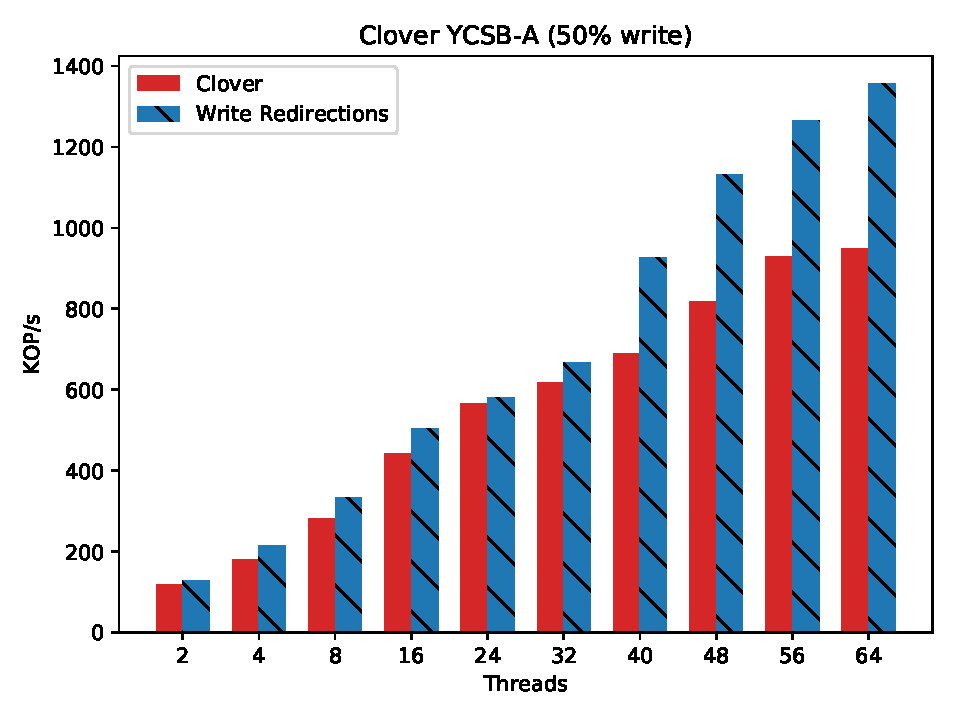
\includegraphics[width=0.45\textwidth]{fig/throughput.pdf}
    \caption{Default Clover throughput vs Clover with write conflict
    detection and correction turned on.}
    \label{fig:throughput}
\end{figure}

\subsection{Memory Consumption}

Resources on networking hardware is scarce. High end SoC SmartNIC's
have just a few GB of RAM, and programmable switches have only MB's of
SRAM. Moreover the use of this memory is not free. Using memory for
any purpose other than buffer packets has a direct performance cost as
the number of packets which can be successfully buffered drops. Our
design takes the preciousness of memory in network into account. The
metadata we cache in network in the minimal necessary to resolve write
conflicts. While Clover's meta data consists of many MB of garbage
collection and version data we only cache the virtual address of the
last write per key. In addition we track the last key written per
client thread. Clients are not explicitly known to our middlebox and
are identified at runtime by their QP. Tracking clients in this way is
necessary to detect write conflicts in clover. This overhead could be
eliminated by explicitly adding key information to CNS requests.

Figure~\ref{fig:memory} Shows the memory overhead as a function of
keys. Note that 100K keys can be supported using 7\% of the available
memory on a Barefoot Tofino programmable switch (22MB).

\begin{figure}
    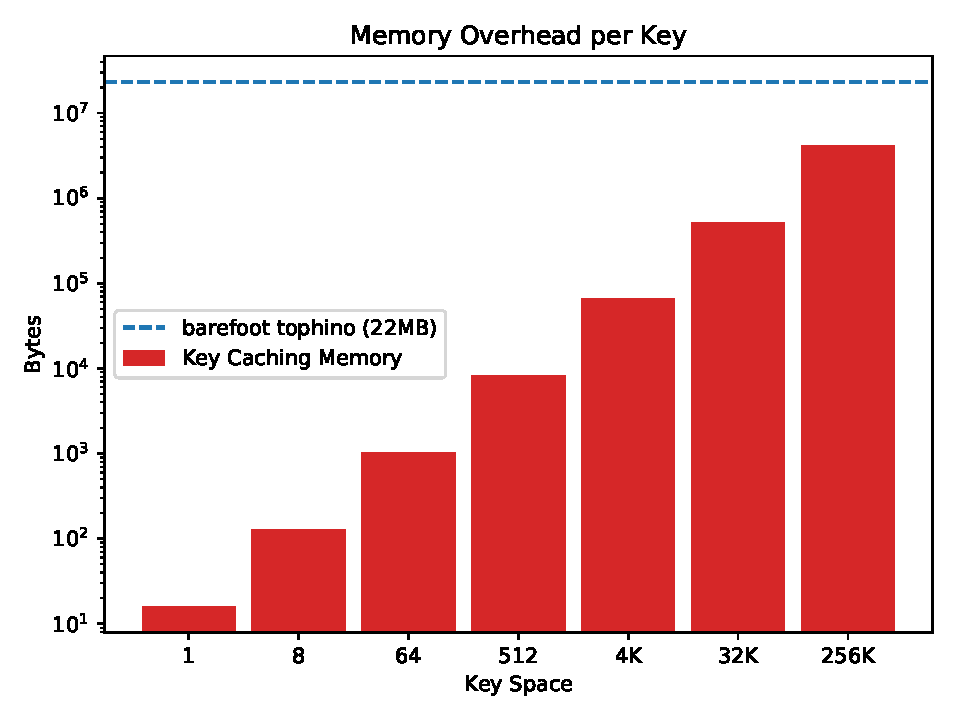
\includegraphics[width=0.45\textwidth]{fig/memory.pdf}
    \caption{Cost of caching metadata in network vs keyspace size.}
    \label{fig:memory}
\end{figure}

\subsection{Caching top \textit{N} keys} 
%%
Hot keys which are written frequently are the most likely to
contribute to conflict. Caching only hot keys results in relatively
large performance gains while requiring only a small portion of the
memory required to cache the entire keyspace. We test the effect of
caching only hot keys by restricting our in network cache to track and
resolve conflicts on only the top \textit{N} keys. In this experiment
RDMA requests for keys which are not caches pass through our middlebox
without modification, conflicts are resolved using Clovers
reconciliation protocol. We ran our experiment with 64 client threads,
with a total keyspace size of 1024 keys. Figure~\ref{fig:cache} shows
the relative throughput gains from caching the top N keys. The request
distribution is zipf(0.75), therefore the vast majority of conflicts
occur on the top 8 keys. The in network memory requirement for 8 keys
is 128 Bytes, which results in 1.3x throughput improvement.

\begin{figure}
    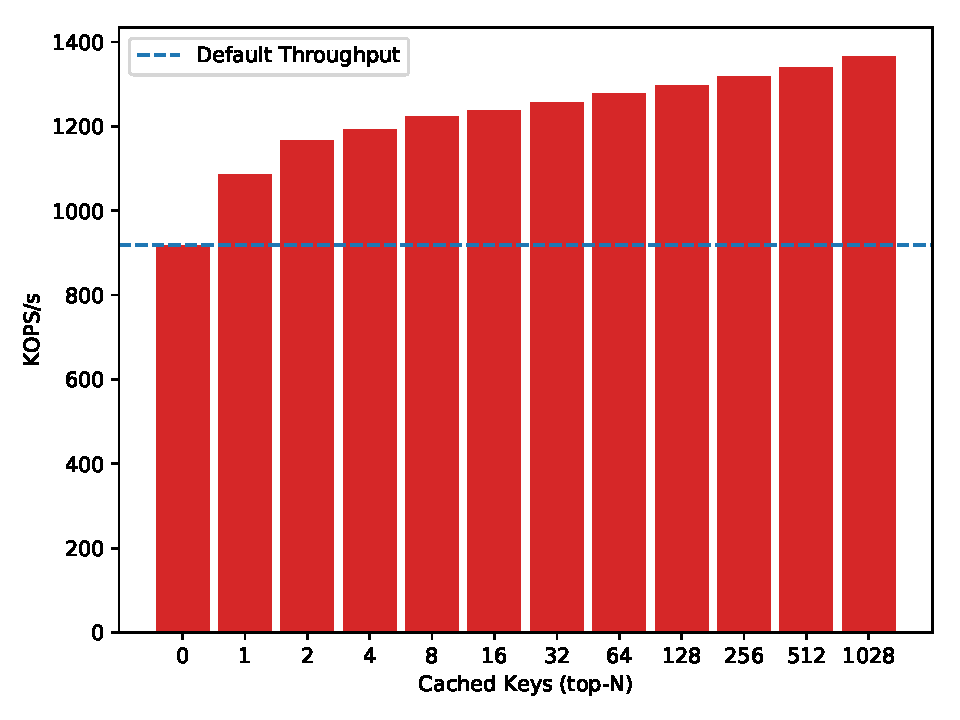
\includegraphics[width=0.45\textwidth]{fig/cache.pdf}
    \caption{Performance as a function of keys cached. Caching a few
    of the top n keys provides the greatest marginal throughput
    benefits.}
    \label{fig:cache}
\end{figure}

\section{Conclusion}

\todo{RDMA write contention}








